    \fontsize{23pt}{24pt}\selectfont
    \textbf{\textcolor{truepurple}{次世代cosplay舞台剧部}}\\
\vspace{0.7em}
  \adjustbox{valign=t}{
    \begin{minipage}[t]{0.25\textwidth}
      \vspace{-0.5em}
      \raisebox{-\height}{
      
\includegraphics[width=\linewidth]{部酱/cosplay舞台剧.png}}
      
      \picbox{\small ~~\ding{115} ~ cosplay舞台剧部酱~}
    \end{minipage}%
    }
    \hfill
    \adjustbox{valign=t}{
    \begin{minipage}[t]{0.65\textwidth}

        \normalsize
    \chind 大家好啊,这里是cosplay舞台剧部!\\
\chind 顾名思义,这里既有cosplay,又有舞台剧———是并集而不是交集。\\
\chind 部门的活动有许多,包括最盛大的社庆舞台剧节目、百团大战出cos、在动漫咖啡厅活动出cos、约漫展、约团片、约计划、约饭……\\
\chind 社庆的舞台剧节目上,我们有19年的命运石之门,21年的方舟走秀,24年的逆转裁判和25年的“苹果默示录”。\\
\chind 在百团大战中,社团会约好c楼的活动室方便大家化妆,一起在摊位上出cos也不社恐。在动漫主题咖啡厅中,我们还会设置符合主题的布景,让大家拍照使用。\\
\chind 大家可以组团去方舟ONLY、V家ONLY等漫展。\\

    
    \end{minipage}
    }
    \adjustbox{valign=t}{
    \begin{minipage}[t]{0.65\textwidth}

        \normalsize

\chind 约团片约计划什么的,只需要在群里说一声。万一成功了呢!这组JOJO黄金之风团片仅仅起源于一句话。并且结束以后一起去吃了披萨。\\
\chind 没出过cos,怎么办?尽管在群里提出问题吧!群内也有技术高超的妆娘、毛娘老师。试着在部门活动中迈出cosplay的第一步。\\
\chind 总之,欢迎所有对此有兴趣的同学加入!
\\  
    
    \end{minipage}
    }
    \hfill
  \adjustbox{valign=t}{
    \begin{minipage}[t]{0.25\textwidth}
      \vspace{-0.5em}
      \raisebox{-\height}{
      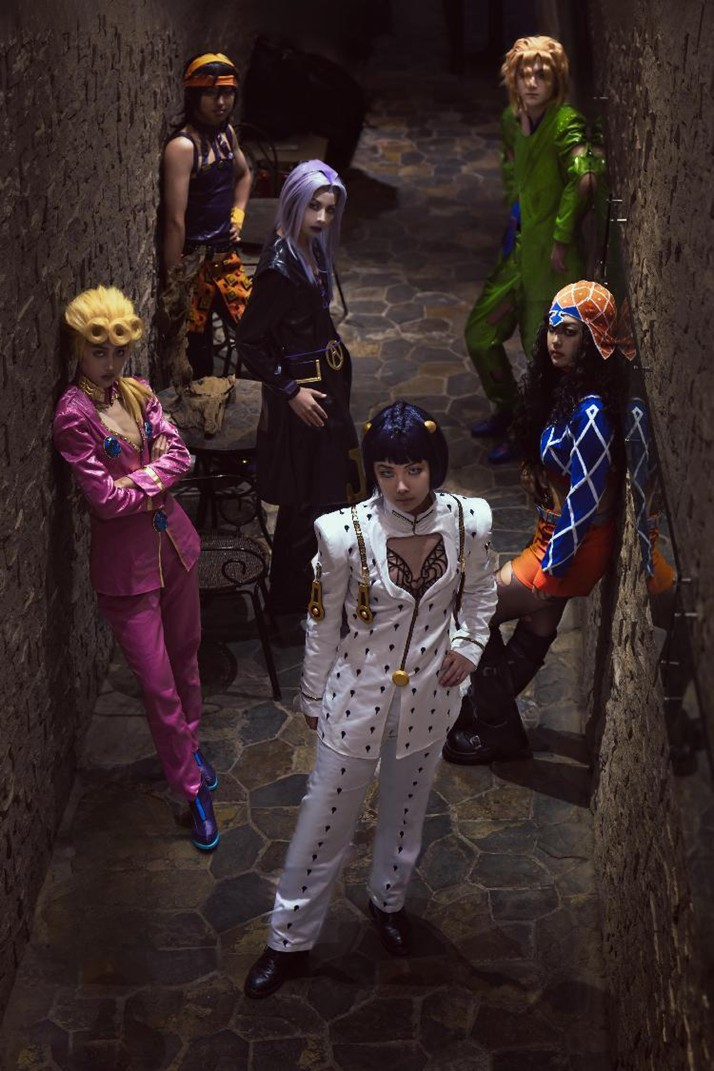
\includegraphics[width=\linewidth]{cos部3.jpg}}
      
      \picbox{\small ~~\ding{115} ~ JOJO黄金之风团片~}
    \end{minipage}%
    }
      \adjustbox{valign=t}{
    \begin{minipage}[t]{0.45\textwidth}
      \vspace{-2.5em}
      \raisebox{-\height}{
      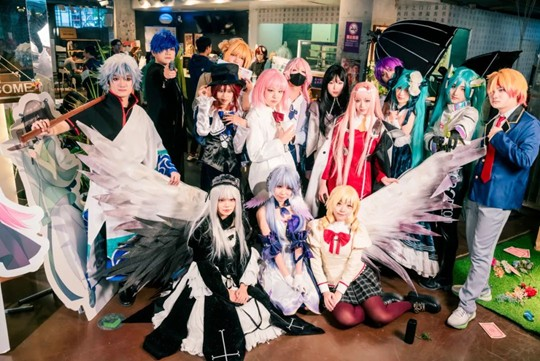
\includegraphics[width=\linewidth]{cos部1.jpg}}
      
      \picbox{\small \ding{115} ~ 2024咖啡厅coser合影~}
    \end{minipage}%
    }  \adjustbox{valign=t}{
    \begin{minipage}[t]{0.45\textwidth}
      \vspace{0.5em}
      \raisebox{-\height}{
      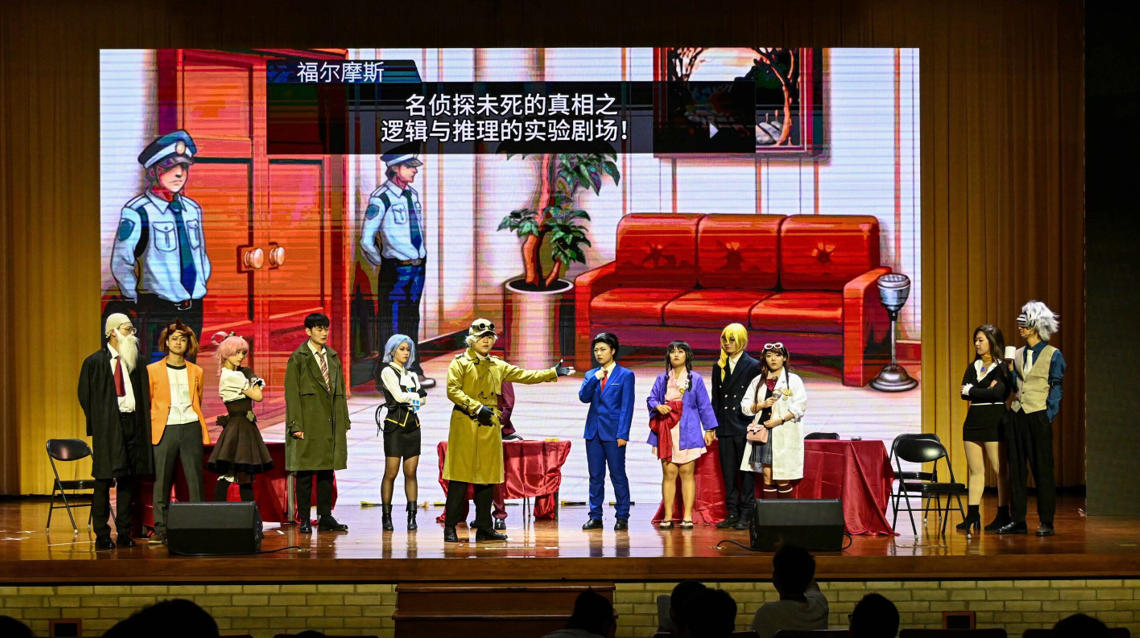
\includegraphics[width=1.1\linewidth]{cos部2.jpg}}
      
      \picbox{\small ~~\ding{115} ~ 2024社庆舞台剧《逆转裁判》~}
    \end{minipage}%
    }
    \newpage
    \fontsize{23pt}{24pt}\selectfont
    \textbf{\textcolor{truepurple}{次世代周边交易部(谷子部)}}\\
  \adjustbox{valign=t}{
    \begin{minipage}[t]{0.25\textwidth}
      
      \raisebox{-\height}{
      
\includegraphics[width=\linewidth]{谷子部1.png}}

    \end{minipage}%
    }
    \hfill
    \adjustbox{valign=t}{
    \begin{minipage}[t]{0.7\textwidth}


        \normalsize
\vspace{0.5em}
\chind “终于上大学了,入坑这么多年,终于能支配财力买点喜欢的周边啦,让我看看——”“诶这个好贵,诶那个怎么像假的,诶这个预定是怎么回事啊”“问题好多不敢下手了o(╥﹏╥)o\ldots”\\
\chind 别急别怕!这里是次世代周边交易部,资深玩家专业团队在线答疑解惑,无论是吧唧爱好者,还是手办收藏家,无论是想打探情报,还是想挥手爆米,都能在这里找到所需所寻☆( ̄▽ ̄)/\$


    
    \end{minipage}
    }
    \normalsize
    \par
    \vspace{0.5em}
\chind 次世代周边交易部,成立于2025.03.10,别名谷子部,顾名思义,我们是一个和\textbf{ACG周边制品}相关、和¥相关的分部,在活跃中展现了极具特色的功能性。
    \adjustbox{valign=t}{
    \begin{minipage}[t]{0.6\textwidth}


        \normalsize

\chind 本部成立的初心,也是本部第一部活,即构建一个和谐实在的\textbf{小二手市场}。
在这里,大家可以按需挂出或收入周边,包括徽章吧唧、立牌、色纸、书籍、
钥匙扣、手办、挂画等现货或预售转单。这里都是自己人,\textbf{可信度高};当面交易,
\textbf{优惠免邮,即时便捷};交流友善,和谐舒心。作为本模块的延伸,
谷子部还会在\textbf{百团展出}各种周边,并在\textbf{咖啡厅同步设置摊位}。

    
    \end{minipage}
    }  
    \hfill
\adjustbox{valign=t}{
    \begin{minipage}[t]{0.35\textwidth}
      
      \raisebox{-\height}{
      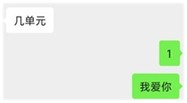
\includegraphics[width=\linewidth]{谷子部2.jpg}}

    \end{minipage}%
    }
    \par
\vspace{0.5em}
\chind 随着部门参与人数增多,依大家所需,谷子部更新出第二部活——\textbf{情报模块}。以资深玩家为中心,谷子部可以为大家提供丰富的\textbf{信息渠道以及购买渠道},为大家\textbf{比价选价,辨别真伪},省钱省心。如各类手办如何购买,如何闲鱼收中古手办,IP限时联动信息,以及BW漫展抢票等等。\\
\chind 在情报模块中,\textbf{线下探店(“开图”)}得到极大的兴趣投入,也自然成为了谷子部第三部活。这一部活中,社友或独行或结伴,去探索城市内各种\textbf{手办店、漫画轻小说店、IP谷子店},足迹遍布京、津、沪、成都、广州、哈尔滨等,最下方为京汇总图及实拍例(上海龙之梦-桐叶pop up,悦荟-深睡羊-异世界情绪展柜)。\\
\chind 周边交易、情报分享、线下开图……谷部活动绝赞上新中,希望大家来一同建设。欢迎各位新老社友加入谷子部,获取更多即时情报\~{}
\par
\adjustbox{valign=t}{
    \begin{minipage}[t]{0.6\textwidth}
      \vspace{0.6em}
      \raisebox{-\height}[0pt][0pt]{
      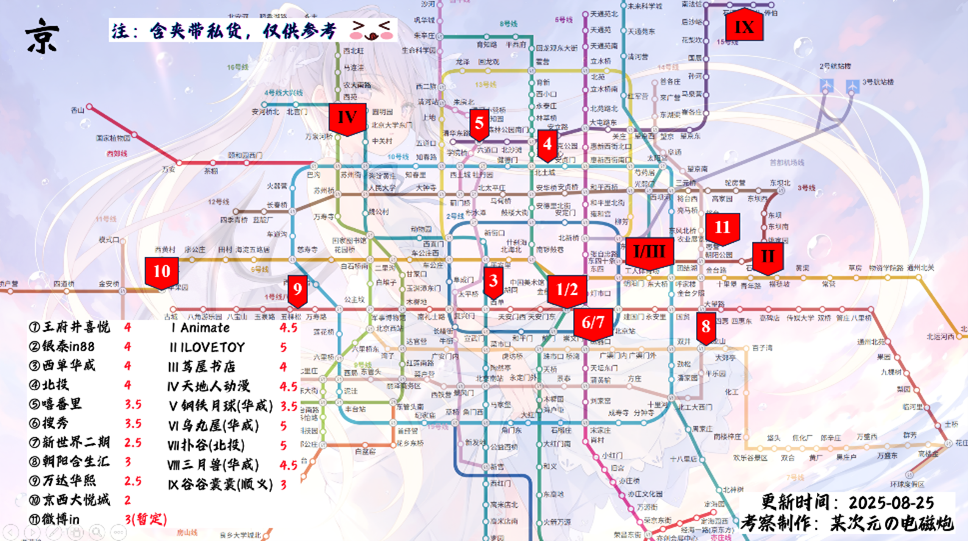
\includegraphics[width=\linewidth]{谷子部3.png}}
    \end{minipage}%
    }
    \hfill
      \adjustbox{valign=t}{
    \begin{minipage}[t]{0.35\textwidth}
      \vspace{-0.5em}
      \raisebox{-\height}{
      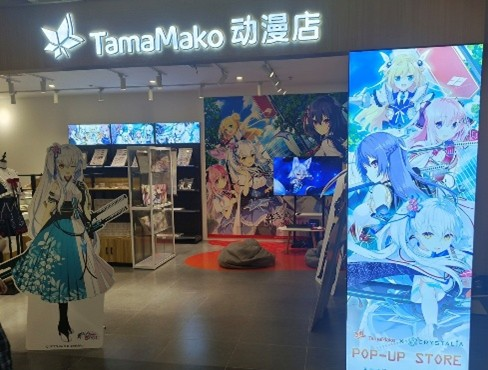
\includegraphics[width=\linewidth]{谷子部4.jpg}}
      \vspace{1em}
      \raisebox{-\height}[0pt][0pt]{
      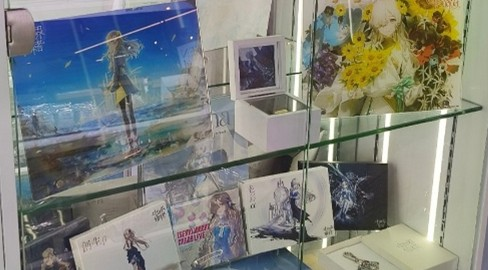
\includegraphics[width=\linewidth]{谷子部5.jpg}}
    \end{minipage}%
    }
\newpage
    \fontsize{23pt}{24pt}\selectfont
    \textbf{\textcolor{truepurple}{次世代水木wota艺部}}\\
    \vspace{0.7em}
  \adjustbox{valign=t}{
    \begin{minipage}[t]{0.3\textwidth}
      \vspace{-0.5em}
      \raisebox{-\height}{
      
\includegraphics[width=1.15\linewidth]{WOTA艺.png}}
      \vspace{-0.5em}
      \picbox{\small ~\ding{115} ~ WOTA艺部酱~}
    \end{minipage}%
    }
    \hfill
    \adjustbox{valign=t}{
    \begin{minipage}[t]{0.6\textwidth}

        \small
\chind wota艺,又称光棒艺,是一项发源于偶像应援文化,发展为独立表演性质的舞蹈形式。
其主要特征为“双脚基本固定,上肢大幅度运动,双手持光棒”。表演形式既可以是视频创作,也可以是舞台表演。\\
\chind wota艺的美感来源于双手所创造出的光弧,以及动作与歌曲节奏的契合度。
只要是你所喜爱的歌曲,就可以由你亲手设计编排,联系部员,带上光棒,
一同对歌曲进行演绎。如果你对舞蹈,MV向视频创作,剪辑与后期感兴趣,
我们欢迎你来探索wota艺这个全新的艺术创作领域。\\
\chind 次世代水木wota艺部最早于2018年创立,自此每年社庆都有节目登台,从未缺席。同时,还参与了诸如社团嘉年华,学生节等多次全校范围的表演活动。与北大元火水月wota艺部常有合作,产出了大量舞台企划和视频企划。此外,与北交,北航,北外,中传等多校均有合作交流。


    
    \end{minipage}
    }
    \par
    \vspace{0.5em}
    \adjustbox{valign=t}{
    \begin{minipage}[t]{0.5\textwidth}

        \small
\chind wota艺部具有丰富的每周常规活动:每周均有2\~{}3次“光棒聚会”,一般在北体二层平台进行,会有手把手的光棒技术教学环节以及视频企划的录制。来时记得带上你最喜欢的歌单,我们会与你共同用光弧演绎!此外还有聚餐,KTV,合宿等项目不定时掉落!\\
\chind 除了社庆以外,wota艺部在次世代宅舞专场和学生节都会有爬台企划,只要每周坚持参加周常,最终都能参与到企划中,登台表演,在聚光灯下展示自我。\\
\chind 如果你对wota艺产生了浓厚的兴趣,想要进一步精进技术,每周末在中关村首钢大平台都有全北京范围的光棒聚会可供参加,可以与领域内最强大的wota艺打师交流学习。北京每年都有2到3次光棒比赛,欢迎参加,证明你的实力!\\
\chind wota艺不仅是表演形式,同时也是一种健康的有氧运动,在锻炼肢体协调能力的同时,提高心肺功能,上肢与核心力量,治疗圆肩驼背,延年益寿,妙处无穷。\\
\chind wota艺更是一种社交方式。在这里,你能找到动漫同好,游戏同好,拓宽交际圈,认识天南海北的朋友,共同享受创作的快乐。\\
\chind 次世代水木wota艺部,欢迎您来!

    \end{minipage}}
    \hfill
    \vspace{1em}
  \adjustbox{valign=t}{
    \begin{minipage}[t]{0.45\textwidth}
      \vspace{-0.5em}
      \raisebox{-\height}{
      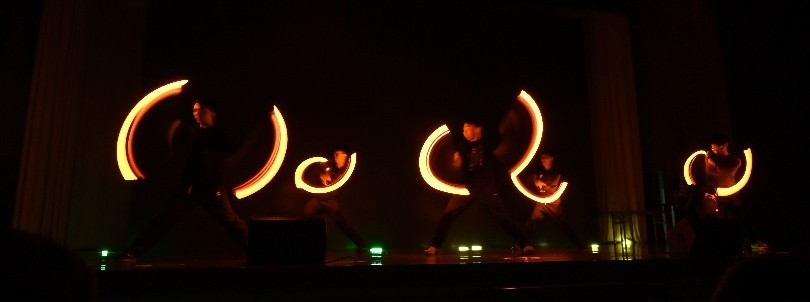
\includegraphics[width=\linewidth]{wota艺部1.jpg}}
      \vspace{-0.5em}
      \picbox{\small ~\ding{115} ~ 软院学生节场照~}
      \begin{minipage}[t]{0.5\textwidth}
        \vspace{-0.5em}
        \raisebox{-\height}{
        
\includegraphics[width=\linewidth]{wota艺部2.png}}
      \end{minipage}%
      \begin{minipage}[t]{0.5\textwidth}
        \vspace{-0.5em}
        \raisebox{-\height}{
        
\includegraphics[width=\linewidth]{wota艺部3.png}}
      \end{minipage}%
        \vspace{-0.5em}
        \picbox{\small ~\ding{115} ~ 与北大水月合作的视频企划\&高考应援企划~}
      \par
      \vspace{-1em}
      \raisebox{-\height}{
      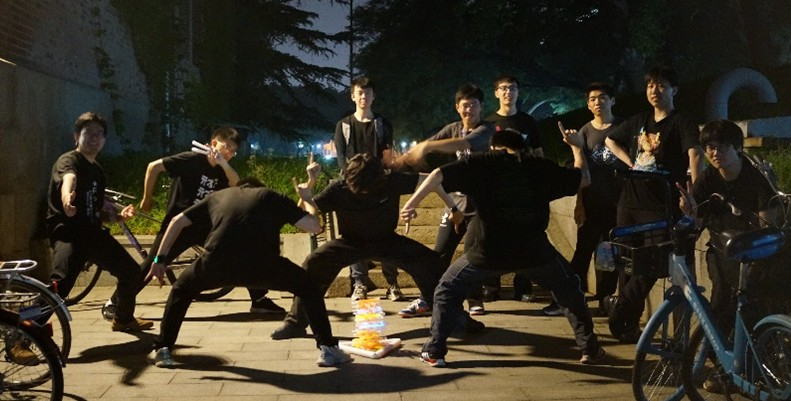
\includegraphics[width=\linewidth]{wota艺部4.jpg}}
      \vspace{-0.5em}
      \picbox{\small ~\ding{115} ~ 神秘合照~}
    \end{minipage}%
    }
 \newpage
\vspace{2em}
  \adjustbox{valign=t}{
    \begin{minipage}[t]{0.2\textwidth}
      \hspace{-1em}
      \raisebox{-\height}{
      
\includegraphics[width=\linewidth]{mc部1.jpg}}
    \end{minipage}%
    }
    \hfill
    \adjustbox{valign=t}{
    \begin{minipage}[t]{0.75\textwidth}
    \fontsize{23pt}{24pt}\selectfont
    \textbf{\textcolor{truepurple}{清华联盟工坊(次世代Minecraft部)}}\\
    \par
    \vspace{-1em}
        \normalsize
清华联盟工坊(THUnion)成立于2019年末,是一个面向清华师生的Minecraft同好会。
THUnion现有成员近800人,目前部门开设有一个原版生存服和一个模组服,
并不定期举办小游戏、建筑大赛、聚餐等丰富多彩的活动。
    \end{minipage}
    }
    \par
    \vspace{1em}

  \adjustbox{valign=t}{
    \hspace{-1.5em}
    \begin{minipage}[t]{0.47\textwidth}
      
      \raisebox{-\height}{
      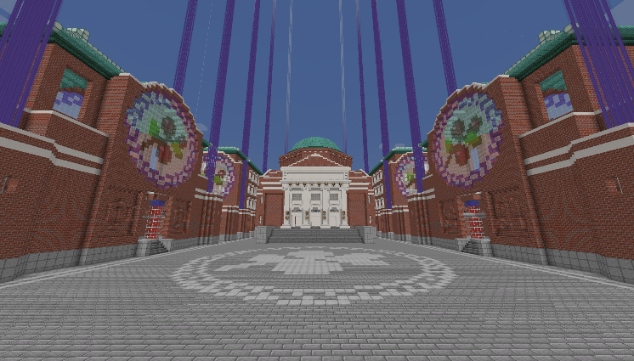
\includegraphics[width=\linewidth]{mc部2.png}}
      \vspace{-0.5em}
      \picbox{\small ~\ding{115} ~ 大礼堂~}
    \end{minipage}%
    }
    \hfill
    \hspace{-1.5em}
  \adjustbox{valign=t}{
    \begin{minipage}[t]{0.47\textwidth}
      
      \raisebox{-\height}{
      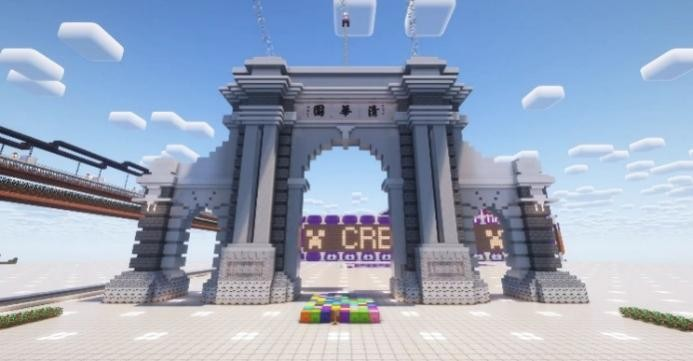
\includegraphics[width=1.095\linewidth]{mc部3.jpg}}
      \vspace{-0.5em}
      \picbox{\small ~\ding{115} ~ 二校门~}
    \end{minipage}
    }
    \par
    \vspace{1em}
  \adjustbox{valign=t}{
    \begin{minipage}[t]{0.47\textwidth}
      \normalsize
\chind 服务器在完善的规章指导下蓬勃发展,建成了矿车洪流凋零骷髅塔、边境恶魂塔、船吸刷怪塔等大型机器;黑石镇、月镇等或雄伟壮丽或精雕细琢的建筑群和上海国际赛车场、维度跑酷等娱乐设施,一片勃勃生机万物竞发的境界。同时部员在游戏机制探索、机器设计领域也取得了许多令人瞩目的成果。例如在部员通力合作下,THUnion成为了世界上首个在1.19+版本实现更新抑制的原版生存服务器。\\
\chind 无论您喜欢玩生存还是生电,建筑还是模组都欢迎加入THUnion和我们一起愉快玩耍!\\
\hspace{-1em}
  \adjustbox{valign=t}{
    
    \begin{minipage}[t]{0.45\textwidth}
      {\raggedright
\scriptsize 即刻扫码加入我们↓ \\[-0.5em](注:为mc部单独审核群)\\[-1em]
}
      
      \raisebox{-\height}{
      
\includegraphics[width=\linewidth]{mc部6.jpg}}

    \end{minipage}%
    }
    \hfill
    \hspace{-1.5em}
  \adjustbox{valign=t}{
    \begin{minipage}[t]{0.4\textwidth}
      \hspace{1em}
      \raisebox{-\height}{
      
\includegraphics[width=1.095\linewidth]{mc部7.jpg}}
      \scriptsize B站扫码关注我们↑

    \end{minipage}
    }
    \end{minipage}
    }
    \hfill
  \adjustbox{valign=t}{
    \begin{minipage}[t]{0.42\textwidth}
      
      \raisebox{-\height}{
      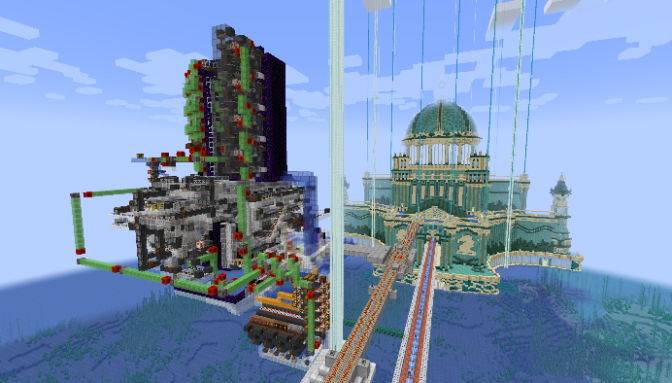
\includegraphics[width=\linewidth]{mc部4.png}}
      \vspace{-0.5em}
      \picbox{\small ~\ding{115} ~ 北海交通枢纽 与 72k泥土机~}
      \raisebox{-\height}{
      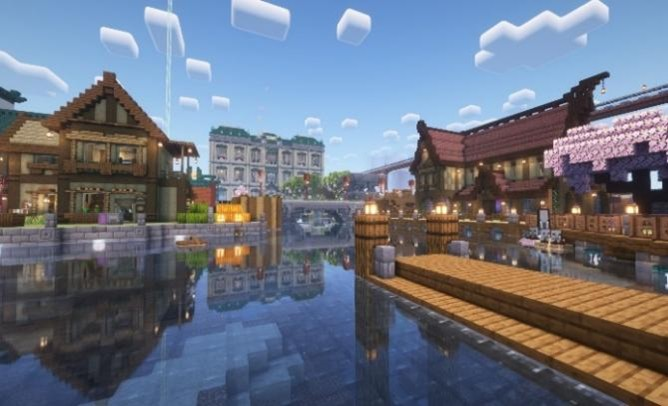
\includegraphics[width=\linewidth]{mc部5.jpg}}
      \vspace{-0.5em}
      \picbox{\small ~\ding{115} ~ 主城金合欢市一角~}
    \end{minipage}
    }


\newpage
    \fontsize{23pt}{24pt}\selectfont
    \textbf{\textcolor{truepurple}{次世代心憩部}}\\
    \vspace{0.7em}
  \adjustbox{valign=t}{
    \begin{minipage}[t]{0.2\textwidth}
      \vspace{-0.2em}
      \raisebox{-\height}[0pt][0pt]{
      
\includegraphics[width=1.1\linewidth]{心憩部.jpg}}
    \end{minipage}%
    }
    \hfill
    \adjustbox{valign=t}{
    \begin{minipage}[t]{0.7\textwidth}

        \small
\chind 欢迎加入心憩部/心理支援部捏!\\
\chind 本部建立的初衷是:互帮互助,让自己的生活更好一些——我们讨论如何改善身心问题与精神困扰,
也欢迎遇到困境的同学群友一起分享从看诊用药心得,到心理调节资源的各种知识,以及日常生活的体验与感想~\\
\chind 为什么会想在次世代动漫社里,建立一个以心理健康为主题的,听上去像抱团取暖(但其实并不是x)的社群呢?\\
\chind 加入次世代一段时间后,我始终忘不了一些社友在一些分部里面,倾诉自己遇到的学习生活困境
,回应他们的却或是无视或是委婉劝止(这里不是讨论沉重话题的地方),或是更多负面悲观的螺旋中。
这样做并不能让现实生活中的问题消失,并且就算有人提出了有价值的信息,也会旋即被水群的日常活动淹没乃至遗忘。\\

    
    \end{minipage}
    }
    \small

    \chind 我希望能真正帮助到大家,我也不认为逃避或者愤世嫉俗才是二次元的主基调,
成长和互帮互助一样是,因此有了这个试图分享心理健康资源,以及提供人文关怀和相互启发的心憩部,
或者也可以叫心理支援部(只是后者可能看起来像是走投无路的同学才会加入的样子,所以改成了前者)\\
\chind \textbf{爱是永不止息,无论在什么地方,以什么方式。}
\\  
    \newpage
    \fontsize{23pt}{24pt}\selectfont
    \textbf{\textcolor{truepurple}{次世代米游杂食铺}}\\
    \vspace{0.7em}
  \adjustbox{valign=t}{
    \begin{minipage}[t]{0.25\textwidth}
      \vspace{-0.2em}
      \raisebox{-\height}[0pt][0pt]{
      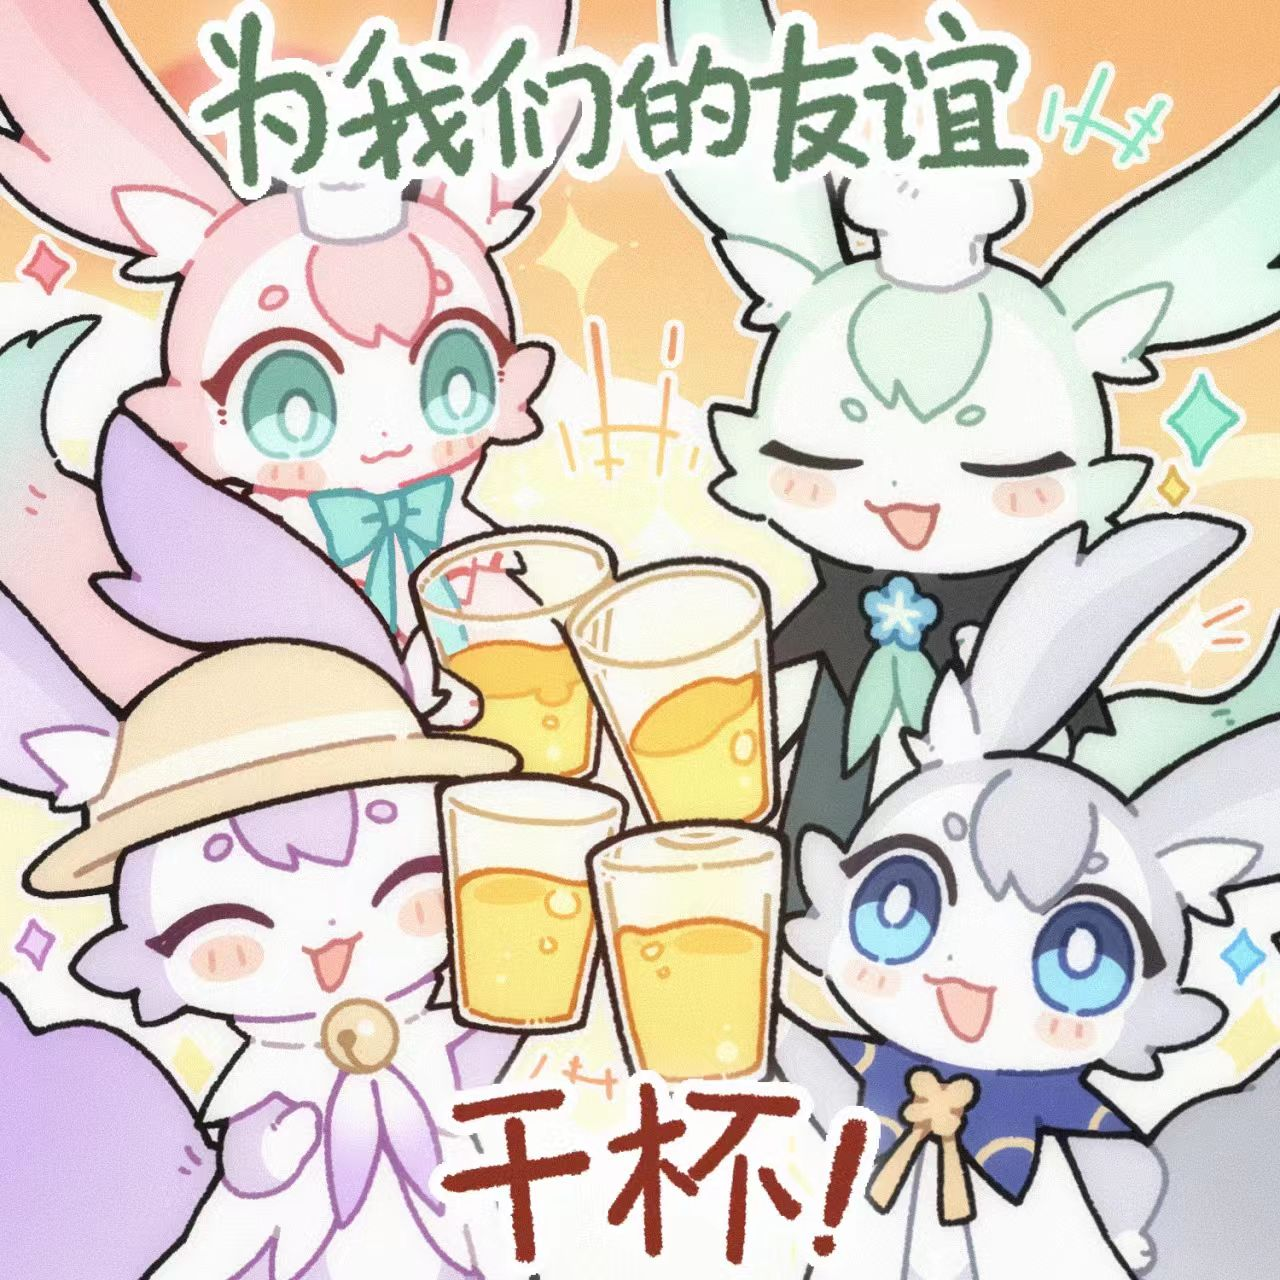
\includegraphics[width=\linewidth]{米游铺1.jpg}}
    \end{minipage}%
    }
    \adjustbox{valign=t}{
    \begin{minipage}[t]{0.65\textwidth}

        \small
\chind 喵喵喵\verb|~~~(^▽^)ゞ| 各位舰长旅行者律师开拓者寻梦者绳匠大家好呀,这里是米家杂食铺!\\
\chind 本部定位为米游社区分层中偏向享受游戏本身而远离焦虑和纷争的部分,所以将对引战/内鬼/拉踩行为做出更加严苛的限制,让我们一起营造出一个mmr友好的小圈吧\~{}\\
\chind 目前群里已有大佬们制作了赛飞儿等AI聊天bot可供大家免费使用,让我们来赛博撸猫吧\~{}\\


    
    \end{minipage}
    }
    \small

\adjustbox{valign=t}{
    \begin{minipage}[t]{0.7\textwidth}

        \small
\chind 此外,本部设立两红包奖项,一为安慰奖,一般在每月所有卡池更新后为群最非颁发约等于一张小月卡的小红包,不要因为抽卡而坏了游戏的性质喔;二为群活跃增值奖,一般在积极参与相关活动并带动群内积极讨论活跃时候颁发。\\  
\chind 欢迎大家来建设部活、分享二创和cos以及各种群帮帮等,让这个小部门热闹起来吧。\\
\chind 所以赶快来加入我们吧\~{}
    \end{minipage}
    }
  \adjustbox{valign=t}{
    \begin{minipage}[t]{0.2\textwidth}
      \vspace{-0.2em}
      \raisebox{-\height}[0pt][0pt]{
      
\includegraphics[width=1.1\linewidth]{米游铺2.jpg}}
    \end{minipage}%
    }
    \hfill

\vspace{2em}    
\fontsize{23pt}{24pt}\selectfont
\textbf{\textcolor{truepurple}{次世代星露谷物语部}}\\
\vspace{0.2em}
\small
\chind 你说得对,但是星露谷物语是一个牧场类的RPG游戏,你继承了爷爷在星露谷的农场,
但是你手头上只有最基础的农具和少许金钱,你得靠此开始你的新生活。
你能把这片杂草丛生的田地变成繁荣的家园吗?\\
\chind 欢迎各位老乡加入,也欢迎感兴趣准备入手的新玩家捏\~{}
